%Kapitel des Hauptteils

\chapter{Lösungsideen}  %Name des Kapitels
\label{cha:Lösungsideen} %Label des Kapitels
%TODO Struktur wie??
In diesem Kapitel werden die Lösungsideen für die Umsetzung der im Kapitel \ref{sec:Zielsetzung} definierten Ziele beschrieben.

\section{Methoden für das OSINT einer ausgewählten Person}
	\subsection{Verwendung von OSINT-Tools}
	Die Personensuche wird durch die Verwendung kostenloser OSINT-Tools durchgeführt.\\ 
	Eine entsprechende Webseite die mehrere OSINT-Methoden bereit stellt, ist unter dem URL \textit{"'https://inteltechniques.com/index.html"'} erreichbar. Sie stellt Methoden zur Suche nach E-Mail-Adressen, Benutzernamen, Social-Media-Profilen, und noch viele mehr zu Verfügung. Allerdings werden nicht nur selbstentwickelt OSINT-Methoden von Michael Bazzell bereitgestellt, sondern auch andere Webseiten mit weiteren OSINT-Tools vorgeschlagen.
	
	\subsection{Algorithmus für OSINT entwickeln}
	Es wird ein Algorithmus für OSINT entwickelt, der aus einem Web Crawler und Web Scraper besteht. Mit diesem ist es möglich eigenständig nach Information zu suchen. Hierfür wird eine Suchmaschine, wie die von Google, verwendet.\\
	Die Suchergebnisse können mit Hilfe des Web Crawlers verfolgt werden. Anschließen wird der Webseitentext, durch den Web Scraper, ausgelesen. Im letzten Schritt, wird der Text analysiert und interpretiert.\\
	All diese Prozesse laufen unabhängig von den vorgeschlagenen Webseiten voll automatisiert ab.


\section{Mögliche Webseiten für OSINT mehrerer unbekannter Personen}
Für das OSINT mehrere unbekannter Personen stehen die Webseiten von FuPa, Xing und LinkedIn zu Auswahl.
	\subsection{XING}
	XING ist ein soziales Netzwerk für Berufstätige mit über 15 Millionen Mitgliedern. Hier vernetzen sich Kontakte aus allen Branchen um Jobs, Mitarbeiter, Aufträge oder ähnliches zu suchen und zu finden.\cite{WasIstXING}\\
	XING bietet allerdings viele Möglichkeiten zum Schutz der Privatsphäre. So kann ein Nutzer einstellen, ob er von einer Suchmaschine gefunden werden oder nur für Xing-Mitglieder sichtbar sein will. %TODO in die Bewertung
	\begin{figure}[H]
		\centering
		
\includegraphics[ scale=0.2]{bilder/XING_profil.png}
		\caption{Profil von der Webseite XING}
		\label{img:XING}
	\end{figure}

	\subsection{LinkedIn}
	LinkedIn ist das weltweit größte soziale Netzwerk für Berufstätige mit mehreren Millionen Mitgliedern. Es vernetzt berufliche Kontakte der ganzen Welt und stellt ebenfalls Möglichkeiten zum Schutz der Privatsphäre zu Verfügung. \cite{WasIstLinkedIn}
	\begin{figure}[H]
		\centering
		
\includegraphics[ scale=0.2]{bilder/LinkedIn_profil.png}
		\caption{Profilkarte von der Webseite LinkedIn}
		\label{img:Linkedin}
	\end{figure}

		\subsection{Fupa}
		Die Webseite Fupa stellt ein regionales Fußballportal dar, welches zur Berichterstattung des Amateurfußballs vorhanden ist. Allerdings werden nicht nur Berichte sondern auch aussagekräftige Spielerprofile zur Verfügung gestellt.\cite{WasIstFUPA} Außer dem verzeichnet FuPa eine Mitgliederzahl von über 200.000.\cite{FuPaMitglieder}\\
		Das Bild \ref{img:FuPa} zeigt ein Spielerprofil, wie es auf dieser Webseite angezeigt wird. Allerdings kann sich die Vollständigkeit eines Profils variieren.
		\begin{figure}[H]
			\centering
			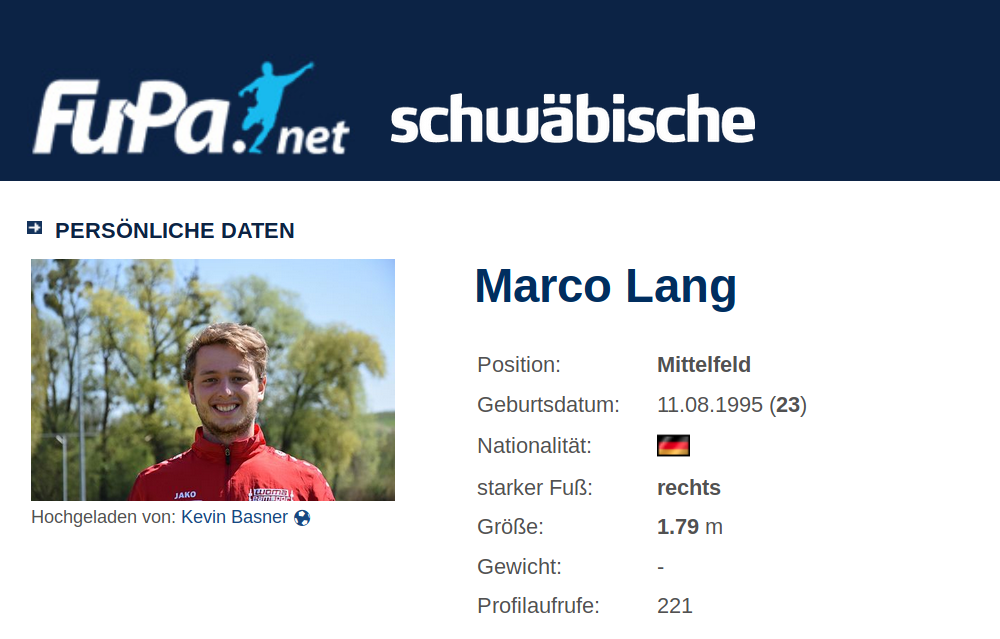
\includegraphics[ scale=0.2]{bilder/fupa_screenshot.png}
			\caption{Spielerprofil von der Webseite FuPa}
			\label{img:FuPa}
		\end{figure}
		%TODO wie viele Mitglieder hat fupa?
	
	\section{Konzept für die Erstellung einer Phishing-Mail}
	Die Generierung einer realen Phishing-Mail benötigt eine korrekte E-Mail-Adresse der Zielperson. Darüber hinaus sollten die gewonnen Informationen in einem sinnvollen E-Mail-Text eingebunden werden. Die Generierung einer Phishing-Mail läuft voll automatisch ab. Das bedeutet, dass das Programm eigenständig die E-Mail-Adressen generiert und passende E-Mail-Muster auswählt.
	
	\subsection{Methoden zur Generierung der E-Mail-Adresse}
	
	Beim OSINT einer ausgewählten Person wird bereits nach E-Mail-Adressen der Zielperson gesucht. Dadurch kann eine bis jetzt unbekannte Anzahl von Adressen gefunden werden. Die Methoden zur Generierung einer E-Mail-Adresse muss dadurch nicht für jede Zielperson durchgeführt werden. In dem Fall, dass keine E-Mail-Adresse gefunden wurde, wird diese Methode verwendet.
	
		\subsubsection{Algorithmus entwickeln zum generieren}
		Es kann ein Algorithmus entwickelt werden, der mögliche E-Mail-Adressen aus den gewonnen Daten generiert. Dies ist durch die Kombination aus Vorname, Nachname, Geburtsjahr und den bekanntesten E-Mail-Providern realisierbar. Für den Fall, dass der Arbeitgeber der Zielperson bekannt ist, kann auf der Firmenwebseite nach E-Mail-Adressen gesucht werden. Dadurch ist es möglich die Domain einer Firmen-Mailadresse zu bestimmen und eine Anzahl möglicher Firmenadressen für die Zielperson zu generieren.\\
		Durch diese Methode wird eine Pool mit möglichen Mailadressen erstellt. Dabei muss jede einzelne E-Mail-Adresse auf Validität geprüft werden.
		%TODO Muss Email auf validität geprüft werden??		
		
		\subsubsection{Automatisierbare OSINT-Tools verwenden}
		Für die Generierung der E-Mail-Adressen kann ein kostenloses OSINT-Tools von Michael Bazzel verwendet werden. Diese Tool ermöglicht es, die gewonnenen Informationen über eine Formular einzugeben. Anschließend werden draus mögliche E-Mail-Adressen generiert. Auch hier entsteht ein Adresspool, bei dem die E-Mail-Adressen auf Validität geprüft werden. Zu dem bringt das Tool eine weitere Funktion mit sich. Es wird automatisch nach Einträgen, der generierten E-Mail-Adressen, im Internet gesucht und angezeigt. \cite{EmailAssumptions}
		
	\subsection{Methoden zur Generierung des E-Mail-Textes}
		\subsubsection{Muster für den E-Mail-Text erstellen}
		\label{subsubsec:EMailMusterMethode}
		Die zu erstellenden E-Mail-Muster entsprechen hier kategorisierten Lückentexten. Abhängig von den gefundenen Daten, wird ein Lückentext ausgewählt und anschließend mit den Daten an den passenden Stellen ergänzt.\\
		Die Lückentexte werden so kategorisiert, dass für jede gefundene Information ein passender Lückentext vorhanden ist. Eine denkbare Unterteilung wären die Kategorien Privat und Geschäftlich.
	
		\subsubsection{E-Mail-Text aus Fragmenten erzeugen}
		\label{subsubsec:EMailTextFragment}
		Bei dieser Methode besteht der E-Mail-Text aus zusammengesetzten Fragmenten. Dafür wird zu jeder gefundenen Information ein Fragment erstellt. Anschließend werden alle Fragmente zu einem Text zusammengefügt. Der Unterschied zur Methode \ref{subsubsec:EMailMusterMethode} besteht darin, dass der E-Mail-Text dynamisch erzeugt wird. Das bedeutet, der endgültige Text ist nicht vorgeben. Er kann aus einer variierenden Anzahl von Fragmenten besteht. Diese Anzahl kann variieren, da sie abhängig von der gefundenen Information über die Zielperson ist.
		
		
		
